\chapter{Costos del Sistema}

 \graphicspath{{Chapter6/Figuras/}{Chapter6/Figs/PDF/}{Chapter4/Figs/}}

En este capítulo se presentan los costos del sistema de reconocimiento de estilo de conducción. Se divide en costos de componentes electrónicos y componentes mecánicos (fabricación de componentes y compra de componentes). Además se considera también un costo de envío como un 40\% del costo de los componentes. Este porcentaje representa los gastos de envío y aduanas, entre otros.

\section{Costos de componentes electrónicos}

Se puede observar en las Tablas \ref{diag:costos_elec_1} y \ref{diag:costos_elec_2} la lista de componentes electrónicos que conforman el sistema de reconocimiento de estilo de manejo con sus costos en dólares.

\begin{table}[htbp!]
  \centering
  \caption{Costo de componentes electrónicos (parte 1)}
  \label{diag:costos_elec_1}
  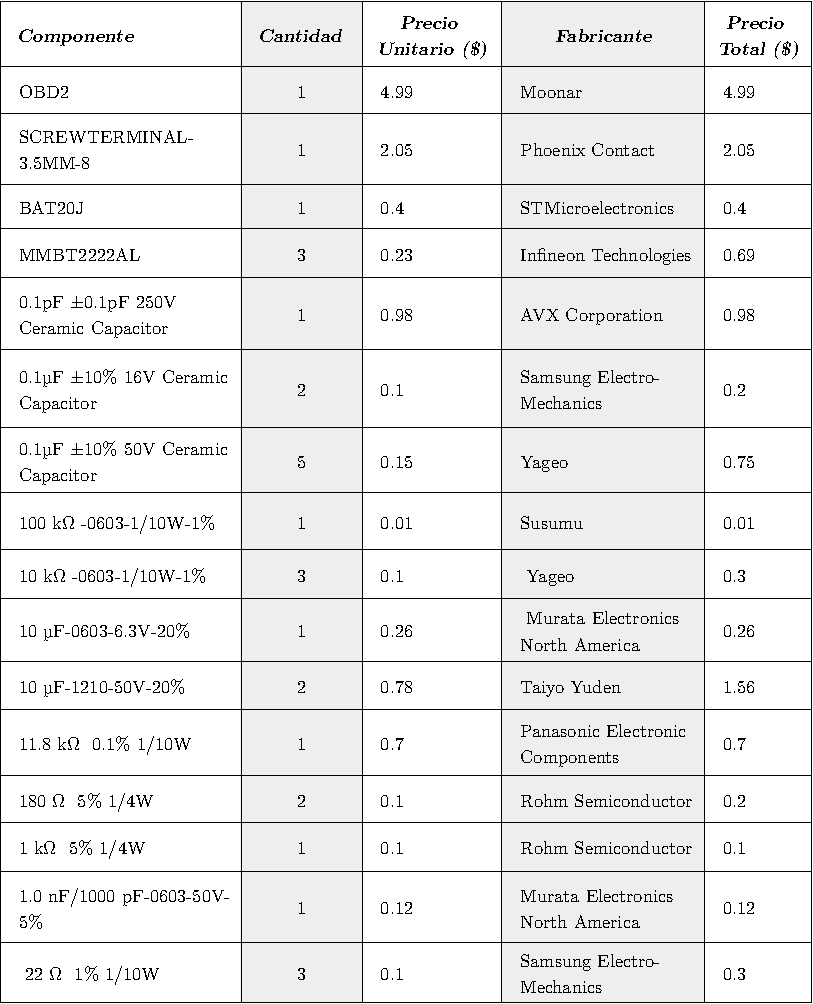
\includegraphics[width=0.9\linewidth]{BOM_1.pdf}
\end{table}

\begin{table}[htbp!]
  \centering
  \caption{Costo de componentes electrónicos (parte 2)}
  \label{diag:costos_elec_2}
  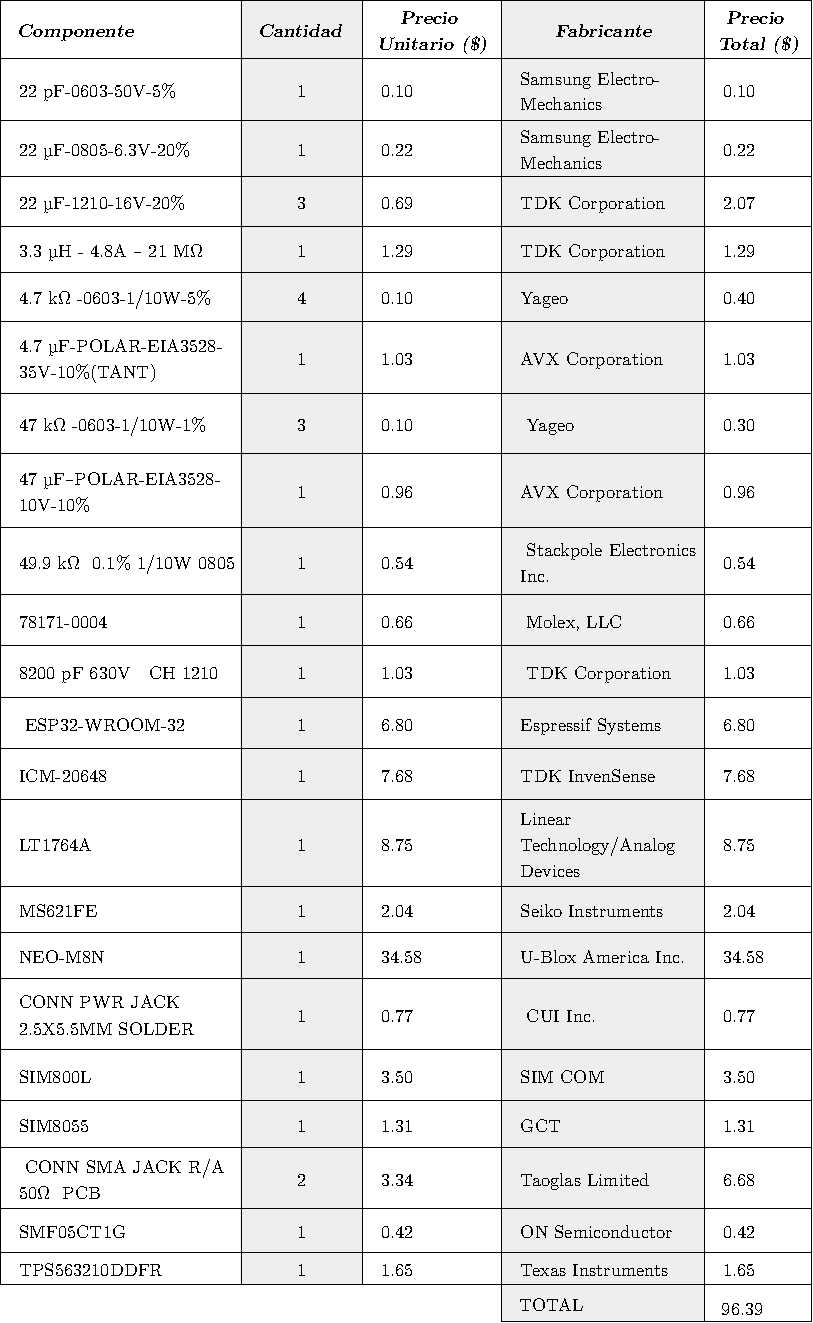
\includegraphics[width=0.9\linewidth]{BOM_2.pdf}
\end{table}

\section{Costos de fabricación y componentes mecánicos}
\section{Costo total}
